% Options for packages loaded elsewhere
\PassOptionsToPackage{unicode}{hyperref}
\PassOptionsToPackage{hyphens}{url}
\PassOptionsToPackage{dvipsnames,svgnames,x11names}{xcolor}
%
\documentclass[
  letterpaper,
  DIV=11,
  numbers=noendperiod]{scrartcl}

\usepackage{amsmath,amssymb}
\usepackage{iftex}
\ifPDFTeX
  \usepackage[T1]{fontenc}
  \usepackage[utf8]{inputenc}
  \usepackage{textcomp} % provide euro and other symbols
\else % if luatex or xetex
  \usepackage{unicode-math}
  \defaultfontfeatures{Scale=MatchLowercase}
  \defaultfontfeatures[\rmfamily]{Ligatures=TeX,Scale=1}
\fi
\usepackage{lmodern}
\ifPDFTeX\else  
    % xetex/luatex font selection
\fi
% Use upquote if available, for straight quotes in verbatim environments
\IfFileExists{upquote.sty}{\usepackage{upquote}}{}
\IfFileExists{microtype.sty}{% use microtype if available
  \usepackage[]{microtype}
  \UseMicrotypeSet[protrusion]{basicmath} % disable protrusion for tt fonts
}{}
\makeatletter
\@ifundefined{KOMAClassName}{% if non-KOMA class
  \IfFileExists{parskip.sty}{%
    \usepackage{parskip}
  }{% else
    \setlength{\parindent}{0pt}
    \setlength{\parskip}{6pt plus 2pt minus 1pt}}
}{% if KOMA class
  \KOMAoptions{parskip=half}}
\makeatother
\usepackage{xcolor}
\setlength{\emergencystretch}{3em} % prevent overfull lines
\setcounter{secnumdepth}{-\maxdimen} % remove section numbering
% Make \paragraph and \subparagraph free-standing
\ifx\paragraph\undefined\else
  \let\oldparagraph\paragraph
  \renewcommand{\paragraph}[1]{\oldparagraph{#1}\mbox{}}
\fi
\ifx\subparagraph\undefined\else
  \let\oldsubparagraph\subparagraph
  \renewcommand{\subparagraph}[1]{\oldsubparagraph{#1}\mbox{}}
\fi


\providecommand{\tightlist}{%
  \setlength{\itemsep}{0pt}\setlength{\parskip}{0pt}}\usepackage{longtable,booktabs,array}
\usepackage{calc} % for calculating minipage widths
% Correct order of tables after \paragraph or \subparagraph
\usepackage{etoolbox}
\makeatletter
\patchcmd\longtable{\par}{\if@noskipsec\mbox{}\fi\par}{}{}
\makeatother
% Allow footnotes in longtable head/foot
\IfFileExists{footnotehyper.sty}{\usepackage{footnotehyper}}{\usepackage{footnote}}
\makesavenoteenv{longtable}
\usepackage{graphicx}
\makeatletter
\def\maxwidth{\ifdim\Gin@nat@width>\linewidth\linewidth\else\Gin@nat@width\fi}
\def\maxheight{\ifdim\Gin@nat@height>\textheight\textheight\else\Gin@nat@height\fi}
\makeatother
% Scale images if necessary, so that they will not overflow the page
% margins by default, and it is still possible to overwrite the defaults
% using explicit options in \includegraphics[width, height, ...]{}
\setkeys{Gin}{width=\maxwidth,height=\maxheight,keepaspectratio}
% Set default figure placement to htbp
\makeatletter
\def\fps@figure{htbp}
\makeatother

\KOMAoption{captions}{tableheading}
\makeatletter
\makeatother
\makeatletter
\makeatother
\makeatletter
\@ifpackageloaded{caption}{}{\usepackage{caption}}
\AtBeginDocument{%
\ifdefined\contentsname
  \renewcommand*\contentsname{Table of contents}
\else
  \newcommand\contentsname{Table of contents}
\fi
\ifdefined\listfigurename
  \renewcommand*\listfigurename{List of Figures}
\else
  \newcommand\listfigurename{List of Figures}
\fi
\ifdefined\listtablename
  \renewcommand*\listtablename{List of Tables}
\else
  \newcommand\listtablename{List of Tables}
\fi
\ifdefined\figurename
  \renewcommand*\figurename{Figure}
\else
  \newcommand\figurename{Figure}
\fi
\ifdefined\tablename
  \renewcommand*\tablename{Table}
\else
  \newcommand\tablename{Table}
\fi
}
\@ifpackageloaded{float}{}{\usepackage{float}}
\floatstyle{ruled}
\@ifundefined{c@chapter}{\newfloat{codelisting}{h}{lop}}{\newfloat{codelisting}{h}{lop}[chapter]}
\floatname{codelisting}{Listing}
\newcommand*\listoflistings{\listof{codelisting}{List of Listings}}
\makeatother
\makeatletter
\@ifpackageloaded{caption}{}{\usepackage{caption}}
\@ifpackageloaded{subcaption}{}{\usepackage{subcaption}}
\makeatother
\makeatletter
\@ifpackageloaded{tcolorbox}{}{\usepackage[skins,breakable]{tcolorbox}}
\makeatother
\makeatletter
\@ifundefined{shadecolor}{\definecolor{shadecolor}{rgb}{.97, .97, .97}}
\makeatother
\makeatletter
\makeatother
\makeatletter
\makeatother
\ifLuaTeX
  \usepackage{selnolig}  % disable illegal ligatures
\fi
\IfFileExists{bookmark.sty}{\usepackage{bookmark}}{\usepackage{hyperref}}
\IfFileExists{xurl.sty}{\usepackage{xurl}}{} % add URL line breaks if available
\urlstyle{same} % disable monospaced font for URLs
\hypersetup{
  pdftitle={Worksheet 1 - DB, R, SQL, Oh My!},
  pdfauthor={Jo Hardin},
  colorlinks=true,
  linkcolor={blue},
  filecolor={Maroon},
  citecolor={Blue},
  urlcolor={Blue},
  pdfcreator={LaTeX via pandoc}}

\title{Worksheet 1 - DB, R, SQL, Oh My!}
\author{Jo Hardin}
\date{2023-01-08}

\begin{document}
\maketitle
\ifdefined\Shaded\renewenvironment{Shaded}{\begin{tcolorbox}[interior hidden, breakable, frame hidden, boxrule=0pt, enhanced, sharp corners, borderline west={3pt}{0pt}{shadecolor}]}{\end{tcolorbox}}\fi

Your Name:
\_\_\_\_\_\_\_\_\_\_\_\_\_\_\_\_\_\_\_\_\_\_\_\_\_\_\_\_\_\_\_\_\_\_

Names of people you worked with:
\_\_\_\_\_\_\_\_\_\_\_\_\_\_\_\_\_\_\_\_\_\_\_\_\_\_\_\_\_\_\_\_\_\_

\begin{itemize}
\item
  Introduce yourself. Which dorm do you live in? What is one great thing
  and one lousy thing about that dorm?
\item
  Name one thing in the Syllabus / website / etc. for this class that
  either sounds strange/unusual or that you would like to know more
  about.
\end{itemize}

\textbf{Task:} Consider a large hospital system that coordinates all
aspects of health care: doctors, visits, prescriptions, surgeries,
billing, etc. Let's say that the hospital has a database which includes
a series of tables linking all the needed information that they
routinely collect.

\begin{enumerate}
\def\labelenumi{\arabic{enumi}.}
\item
  Come up with at least five tables which might exist in the hospital
  database. For each table indicate a few columns / variables.
\item
  Draw arrows between the tables and indicate the variable(s) that link
  the tables. No table should be completely isolated.
\end{enumerate}

\newpage

\textbf{Solution:}

The solution is taken directly from w3resource. Consider the
hypothetical SQL schema diagram in Figure~\ref{fig-hosp-db}. Some of the
tables and respective variables are described below.

\begin{itemize}
\tightlist
\item
  \texttt{physician}

  \begin{itemize}
  \tightlist
  \item
    employeeid - unique ID of a physician
  \item
    name - name of physician
  \item
    position - designation of a physician
  \item
    ssn - social security number of physician
  \end{itemize}
\item
  \texttt{department}

  \begin{itemize}
  \tightlist
  \item
    departmentid - unique ID of the department
  \item
    name - name of the department
  \item
    head - ID of the physician who is the head of the department,
    connects to the employeeid of the table physician
  \end{itemize}
\item
  \texttt{affiliated\_with}

  \begin{itemize}
  \tightlist
  \item
    physician - ID of the physician, connects to the employeeid of the
    table \texttt{physician}
  \item
    department - ID of the department, connects to the departmentid of
    the table \texttt{department}
  \item
    primaryaffiliation - logical column which indicates whether the
    physicians are affiliated or not
  \end{itemize}
\item
  \texttt{procedure}

  \begin{itemize}
  \tightlist
  \item
    code - unique ID of the medical procedure
  \item
    name - name of the medical procedure
  \item
    cost - cost of the medical procedure
  \end{itemize}
\item
  \texttt{trained\_in}

  \begin{itemize}
  \tightlist
  \item
    physician - ID of the physician, connects to the employeeid of the
    table \texttt{physician}
  \item
    treatment - ID of the medical procedure, connects to the code of the
    \texttt{procedure} table
  \item
    certificationdate - starting date of certification
  \item
    certificationexpires - expiry date of certification
  \end{itemize}
\item
  \texttt{patient}

  \begin{itemize}
  \tightlist
  \item
    ssn - unique ID for each patient
  \item
    name - name of patient
  \item
    address - address of patient
  \item
    phone - phone number of patient
  \end{itemize}
\end{itemize}

\begin{figure}

{\centering 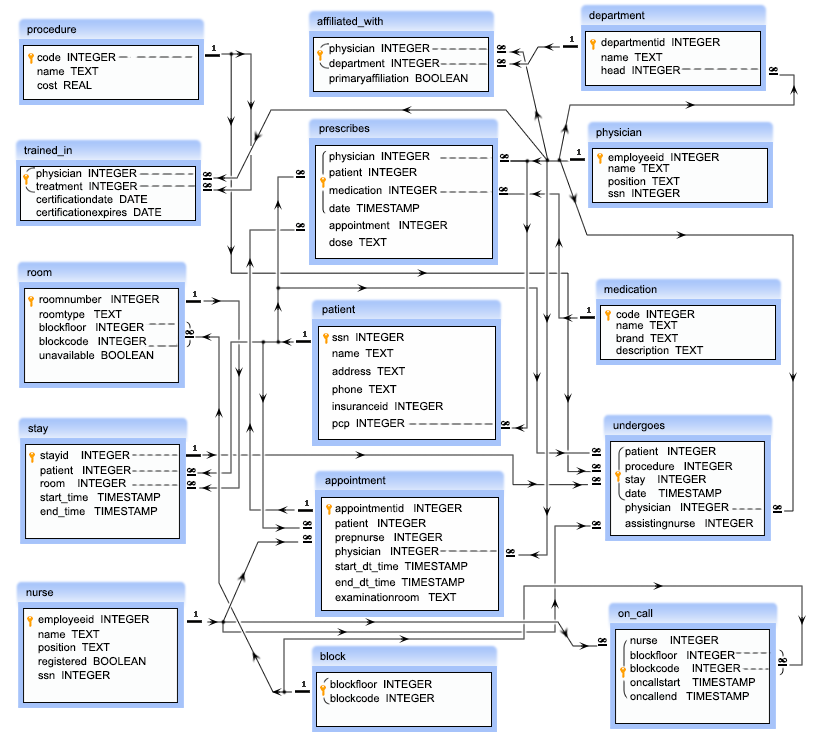
\includegraphics[width=0.9\textwidth,height=\textheight]{../images/hospital-database.png}

}

\caption{\label{fig-hosp-db}SQL schema describing links of tables from a
hypothetical hospital database, image credit:
https://www.w3resource.com/sql-exercises/hospital-database-exercise/index.php}

\end{figure}



\end{document}
